% -*- coding:utf-8 -*-
\documentclass[12 pt, a4paper, twoside]{article}

\usepackage[utf8]{inputenc}
\usepackage[T1]{fontenc}
\usepackage[spanish, activeacute]{babel}
\usepackage[pdftex, bookmarks, hyperfootnotes=false, colorlinks=true,%
            urlcolor=blue, linkcolor=black,  citecolor=black,%
            pagecolor=black, anchorcolor=black, breaklinks=true]{hyperref}
\usepackage{times}
\usepackage{eurosym}
\usepackage{hyperref}

\usepackage[pdftex]{graphicx}
%\usepackage{rotating}
\graphicspath{{img/}}

\usepackage{epstopdf}
\epstopdfsetup{outdir=img/,
  suffix=-generated}

\usepackage[pdftex]{color}
\definecolor{gray97}{gray}{.97}
\definecolor{gray75}{gray}{.75}
\definecolor{gray45}{gray}{.45}

\usepackage{listingsutf8}
\lstset{
  inputencoding = utf8/latin1,
                  %
                  frame = Ltb,
                  framerule = 0 pt,
                  aboveskip = 0.5 cm,
                  framextopmargin = 3 pt,
                  framexbottommargin = 3 pt,
                  framexleftmargin = 0.4 cm,
                  framesep = 0 pt,
                  rulesep = .4 pt,
                  backgroundcolor = \color{gray97},
                  rulesepcolor = \color{black},
                  %
                  stringstyle = \ttfamily,
                  showstringspaces  =  false,
                  basicstyle = \small\ttfamily,
                  commentstyle = \color{gray45},
                  keywordstyle = \bfseries,
                  %
                  numbers = left,
                  numbersep = 15 pt,
                  numberstyle = \tiny,
                  numberfirstline  =  false,
                  breaklines = true
}

\hypersetup{colorlinks = true, urlcolor = blue,
            pdftitle = Game Design Document,
            pdfsubject = Práctica de Ingeniería del Software II,
            pdfauthor = Varios}

\hoffset -0.54 cm
\voffset -0.54 cm
\textheight = 22 cm
\textwidth = 17 cm
\topmargin = 0 cm
\oddsidemargin = 0 cm
\evensidemargin = 0 cm
%\parindent = 0 cm
\parskip = 6 pt

\usepackage{fancyhdr}
\pagestyle{fancy}
\fancyhf[EH,EF,OH,OF]{}
\fancyhf[OLH]{Práctica 2}
\fancyhf[ERH]{Ingeniería del Software 2011-12}
\fancyhf[ELH]{\thepage}
\fancyhf[ORH]{\thepage}

\pdfimageresolution = 300

% \title{Práctica 2: {\em Game Design Document}\\Ingeniería del Software 2011-12}
% \author{Manuel José Abaldea García-Pliego\\
% Luis Miguel Garcia-Muñoz Pérez\\
% Eduardo Monroy Martínez\\
% Felipe Terriza García-Muñoz}
% \date{}

\begin{document}

%\maketitle

\begin{titlepage}
\begin{center}

\begin{figure}[h]
\centering

\includegraphics[width = 12 cm]{esi_color.eps}
\end{figure}

{\huge Ingeniería del Software II 2011-12.\\}

{\huge Desarrollo de una aplicación en Android.\\}
\end{center}

\begin{center}
29 de Abril del 2012
\end{center}

\begin{center}
{\large Manuel José Abaldea García-Pliego

Luis Miguel Garcia-Muñoz Pérez

Eduardo Monroy Martínez

Felipe Terriza García-Muñoz}
\end{center}

\end{titlepage}


\newpage

\tableofcontents

\newpage

\section{Sobre Android y las tecnologías utilizadas}
\subsection{Android}
\subsubsection{Introducción}
Android constituye una pila de software pensada para dispositivos móviles y
que incluye tanto un sistema operativo, como middleware y diversas aplicaciones
de usuarios. Google Inc. desarrolla Android en noviembre de 2007, aunque
posteriormente un conglomerado de empresas agrupadas bajo el nombre de Open
Handset Alliance (OHA), se une al proyecto. Desde su lanzamiento, son muchos
los programadores que han confiado en Android como plataforma de desarrollo de
sus aplicaciones para dispositivos móviles por características como la sencillez y
el gran número de funcionalidades.

Como características generales conviene mencionar que Android está basado en
el núcleo de Linux 2.6, tiene licencia de distribución Apache, convirtiéndolo así en
software libre. Todas las aplicaciones para Android se programan en lenguaje Java
y se ejecutan en una máquina virtual diseñada para esta plataforma denominada
Dalvik.

A lo largo de este trabajo se describirán las características técnicas de Android,
deteniéndose en las partes fundamentales de que consta su arquitectura. Se recogerán
algunas de las principales herramientas de desarrollo y depuración y se
explicará la forma de publicar las aplicaciones Android. Por último, se citarán
algunos de los dispositivos Android y se establecerá una comparativa con otros
sistemas operativos para móviles.

\subsubsection{Características técnicas de Android}
Las características técnicas que posee Android son las siguientes:
\begin{itemize}
\item Framework de aplicaciones: permite reutilización y reemplazo de
  componentes.
\item Máquina virtual Dalvik: optimizada para dispositivos móviles.
\item Navegador integrado: basado en el motor de código abierto
  WebKit.
\item Gráficos optimizados, con una biblioteca de gráficos 2D; gráficos 3D basado
en la especificación OpenGL ES 1.0 (aceleración por hardware
opcional).
\item SQLite para almacenamiento de datos estructurados.
\item Soporte para medios con formatos comunes de audio, vídeo e imágenes
planas (MPEG4, H.264, MP3, OGG, AAC, AMR, JPG, PNG, GIF).
\item Telefonía GSM (dependiente del hardware).
\item Bluetooth, EDGE, 3G, y WiFi (dependiente del hardware).
\item Cámara, GPS, brújula, inclinómetro y acelerómetro (dependiente del
hardware).
\item Ambiente rico de desarrollo incluyendo un emulador de dispositivo, herramientas
para depurar, perfiles de memoria y rendimiento, y un complemento
para el IDE Eclipse.
\item Pantalla táctil.
\item Android Market permite que los desarrolladores pongan sus aplicaciones,
gratuitas o de pago, en el mercado a través de esta aplicación accesible desde
la mayoría de los teléfonos con Android.
\item A continuación se especificarán las versiones y se describirá la arquitectura de
Android.
\end{itemize}

\subsubsection{Versiones de android}
\begin{center}
  \includegraphics[width = 10 cm]{img/figura1.jpg}
\end{center}
La version actual de android es la 4.0 (Ice Cream Sandwich):

Versión que unifica el uso en cualquier dispositivo, tanto en
teléfonos, tablets, televisores, netbooks, etc.

Interfaz limpia y moderna con una nueva fuente llamada "Roboto", muy
al estilo de Honeycomb.

Opción de utilizar los botones virtuales en la interfaz de usuario, en
lugar de los botones táctiles capacitivos.

Llega la aceleración por hardware, lo que significa que la interfaz
podrá ser manejada y dibujada por la GPU y aumentando notablemente su
rapidez, su respuesta y evidentemente, la experiencia de usuario.

Multitarea mejorada, estilo Honeycomb. Añadiendo la posibilidad de finalizar una tarea simplemente desplazándola fuera de la lista.
Ha añadido un gestor del tráfico de datos de internet. El entorno le
permite establecer alertas cuando llegue a una cierta cantidad de uso
y desactivación de los datos cuando se pasa de su límite.

Los widgets están en una nueva pestaña, que figuran en una lista
similar a las aplicaciones en el menú principal.

El corrector de texto ha sido rediseñado y mejorado, ofreciendo la
opción de tocar en una palabra para que nos aparezca una lista con las
diferentes opciones de edición y sugerencias de palabras similares.

Las notificaciones tiene la posibilidad de descartar las que no son
importantes y también desplegar la barra de notificaciones con el
dispositivo bloqueado.

La captura de pantalla, con solo pulsando el botón de bajar volumen y
el botón de encendido.

La aplicación de la cámara se ha llevado un buen lavado de cara, con
nuevas utilidades como es la posibilidad de hacer fotografías
panorámicas de forma automática.

Android Beam es la nueva característica que nos permitirá compartir
contenido entre teléfonos. Vía NFC (Near Field Communication).

Reconocimiento de voz del usuario.

Aplicación de teléfono nuevo con la funcionalidad de buzón de voz
visual que le permite adelantarlo o retroceder los mensajes de voz.

Reconocimiento facial, lo que haría que puedas cambiar la vista.

Las carpetas son mucho más fáciles de crear, con un estilo de
arrastrar y soltar.

Un único y nuevo framework para las aplicaciones.

El usuario tendrá herramientas para ocultar y controlar las
aplicaciones que nos ``cuelgue'' la operadora de turno o el
fabricante, liberando recursos de segundo plano (ciclos de ejecución y
memoria ram). No obstante, no se podrán desinstalar.

Soporte nativo del contenedor MKV.

Soporte nativo para el uso de Stylus (lápiz táctil).

\begin{center}
  \includegraphics[width = 10 cm]{img/figura1_1.jpg}
\end{center}

Con todo esto, Android persigue mejorar y estandarizar el desarrollo de aplicaciones
para dispositivos móviles, reuniendo en la misma plataforma todos los
elementos para acceder a cualquier tipo de funcionalidad en estos dispositivos
(cámara, bluetooth, Wi-Fi, videojuegos, etc.) y añadiendo nuevos servicios como
los que ofrece la web, sin perder de vista en ningún momento la portabilidad
(intentando evitar la fragmentación presente en otras plataformas que actualmente
existen en el mercado) y la reusabilidad.

\subsubsection{Arquitectura de Android}
La arquitectura de esta plataforma está organizada en capas. Cada capa usa los
servicios de las capas inferiores y, a su vez, presta servicios a las capas superiores.
Se distinguen las siguientes capas:
\begin{itemize}
\item Aplicaciones. Incluyen un cliente de e-mail, programa de SMS, calendario,
mapas, navegador, contactos, etc. Todas las aplicaciones están escritas en el
lenguaje Java.
\item Framework de aplicaciones. También escrito en Java, es el conjunto de
herramientas de desarrollo de cualquier aplicación. Todas las aplicaciones
Android usan las mismas APIs del framework. A su vez, los desarrolladores
de aplicaciones pueden acceder a todo el código fuente de las aplicaciones,
fomentando así la reusabilidad.
\item Librerías. Están escritas en C/C++. Los desarrolladores acceden a estas
librerías a través del framework de aplicaciones. Algunas de las más importantes
son libc (incluye cabeceras y funciones según el estándar del lenguaje
C), SQLite (creación y gestión de bases de datos relacionales), OpenGL/SL
y SGL (proporcionan la capacidad gráfica), Surface Manager (gestiona las
ventanas abiertas y los elementos de navegación de la pantalla activa), Media
Libraries (proporciona los códecs para el soporte de contenido multimedia),
etc.
\item Runtime de Android. Lo constituyen las Core Libraries (librerías con
multitud de clases Java) y la máquina virtual Dalvik.
Núcleo de Linux. Android emplea el núcleo de Linux 2.6 para dar soporte
al hardware presente en los dispositivos móviles. Es código abierto, con lo
que se respeta la licencia Apache y ofrece multitud de drivers.
\end{itemize}

Esta arquitectura se aprecia en la figura 2:
\begin{center}
  \includegraphics[width = 10 cm]{img/figura2.jpg}
\end{center}

\textbf{Ciclo de vida de las aplicaciones Android:}
Cada aplicación se ejecuta en su propio proceso. Android se encarga de la
gestión de procesos (creación, eliminación, etc.) de forma transparente al usuario.
Cada proceso (que se corresponde con una aplicación) está formado por una o varias
actividades independientes (componente Activity). Para pasar de una actividad
a otra, Android duerme el proceso, que será despertado cuando sea necesario. Las
acciones que se llevan a cabo sobre las actividades son las siguientes:
onCreate(). Representa la creación de la actividad.
onDestroy(). Representa el fin de la actividad.
onStart(). Representa el inicio de la visibilidad de la aplicación. No es
necesario que la aplicación tenga el foco de acción.
onStop(). Representa el fin de la visibilidad de la aplicación.
onResume(). Representa el inicio de la parte útil de la vida de la aplicación.
Ésta tiene el foco de acción y permite que el usuario interactúe. En este
estado se puede decir que el proceso está despierto.
onPause(). Representa el fin de la parte útil de la vida de la aplicación. En
este estado se puede decir que el proceso está dormido.

\begin{center}
  \includegraphics[width = 10 cm]{img/figura3.jpg}
\end{center}

Un proceso puede ser eliminado cuando está en estado onStop() o onPause().
El proceso eliminado puede ser restaurado si fuera necesario gracias a una copia.
Si no existen recursos suficientes, es necesario eliminar procesos. Android prioriza
los procesos, eliminando en primer lugar los de menor prioridad. La jerarquía que
emplea, listada en orden decreciente de prioridad es la siguiente:
Procesos en primer plano. Son necesario para lo que el usuario está realizando
actualmente (tienen algún componente Activity ejecutándose con
el que el usuario interactúa, tiene un componente Broadcast Intent
Receiver ejecutándose o ha lanzado otro proceso que actualmente tiene un
Service en ejecución).
Procesos visibles. Tiene un componente Activity en la pantalla, pero a
diferencia de los anteriores, el usuario no está interactuando con él.
Procesos de servicio. Son procesos con un componente Service.
Procesos en segundo plano. Son procesos con una o varias Activities
que no son visibles al usuario.
Procesos vacíos. No ejecutan ninguna actividad. Se mantienen en memoria
para agilizar una posible restauración.

\subsubsection{Herramientas de Android}
El SDK de Android incluye muchas herramientas que facilitan la creación de
aplicaciones. Las más importantes son las que se recogen a continuación:
Emulador. Es junto con el plugin ADT, la herramienta más importante
de Android. Permite el diseño, depuración y prueba de las aplicaciones en
el entorno de ejecución de Android. Alguna de sus múltiples opciones se
explicarán a continuación.
Plugin ADT. Es un plugin integrable en Eclipse que facilita la creación de
aplicaciones Android.
Android Virtual Devices (AVDs). Son los dispositivos empleados por el
emulador para ejecutar las aplicaciones. Permiten configurar la plataforma y
otras opciones hardware, así como emplear diferentes skins para el emulador.
Dalvik Debug Monitor Service (DDMS). Está integrada en la máquina virtual
Dalvik y ayuda en la depuración, al permitir la finalización de procesos,
la selección de otros para la depuración y la generación de información de
trazas, entre otras opciones.
Android Debug Bridge (ADB). Entre sus funciones más importantes, está
la de permitir instalar los archivos .apk de las aplicaciones en un emulador y
acceder a estas desde línea de comandos.
Android Asset Packaging Tool (APPT). Permite crear los archivos .apk
que posteriormente será el que se encuentre en el dispositivo móvil.
mksdcard. Ayuda en la creación de una imagen de disco que se puede usar
en el emulador para simular la presencia de una tarjeta de almacenamiento
externa (como una SD).
dx. Convierte el bytecode (archivos .class) en Android bytecode (archivos
.dex).

\textbf{Emulador de Android:}

Como se acaba de indicar, el emulador permite probar y depurar de forma
eficiente las aplicaciones desarrolladas. Emula un dispositivo real mediante el uso
de un AVD. Además de tener aplicaciones preinstaladas y cambiar las distintas
skins, ofrece, entre otras múltiples opciones, la posibilidad de interactuar con él a
través de Telnet. El emulador se puede lanzar desde línea de comandos ejecutando
emulator -avd <avd\_name>, o a través de la ejecución de cualquier aplicación
en Eclipse. El emulador simula un procesador ARM y permite la simulación de
eventos como el envío de SMS o llamadas entrantes. Así, una vez lanzado un
emulador, se le pueden enviar órdenes mediante Telnet conectándose al puerto en
el que se encuentra (por defecto y para la primera instancia es el 5554). Entre las
órdenes más significativas se pueden distinguir las siguientes:
\begin{itemize}
\item help. Imprime la lista de comandos disponibles.
\item event. Envía distintos eventos al emulador.
\item geo. Establece una localización mediante coordenadas GPS.
\item gsm. Emula llamadas telefónicas.
\item kill. Finaliza la instancia del emulador.
\item network. Configura aspectos de red GSM, GPRS, UMTS, etc.
\item power. Controla el nivel de batería.
\item quit|exit. Cierra la conexión establecida con el emulador.
\item redir. Redirecciona puertos de conexión con el emulador.
\item sms. Envía mensajes SMS al emulador.
\item avd. Controla el dispositivo AVD.
\item window. Configura el skin del emulador.
\end{itemize}
Los pasos de conexión por Telnet a un AVD y el envío de un SMS y una
llamada posterior se muestra a continuación:
Lanzar un emulador tal y como se explicó anteriormente, preferiblemente
desde Eclipse.
Ejecutar en un terminal:
\begin{center}
  \includegraphics[width = 10 cm]{img/figura4.jpg}
\end{center}
La razón del empleo del comando redir es redireccionar las conexiones tcp en
este caso con el puerto 5000 al 6000 para evitar las restricciones del router del
emulador.
Para enviar un mensaje, se emplea el formato sms send <phonenumber><text\_message>.
En caso de ejecutar sms send 123 «Enviando el primer mensaje al emulador
de Android», el resultado es el siguiente:
\begin{center}
  \includegraphics[width = 10 cm]{img/figura5.jpg}
\end{center}

Para realizar la llamada posterior se emplea el formato gsm call <phonenumber>,
por ejemplo, gsm call 123. La recepción de la llamada se muestra a
continuación:
\begin{center}
  \includegraphics[width = 10 cm]{img/figura6.jpg}
\end{center}

Se ofrecen opciones de comunicación entre dos emuladores en la página web
http://developer.android.com/guide/basics/what-is-android.
html en la sección Interconnecting Emulator Instances.

\textbf{Dalvik Debug Monitor Service}
Como se comentó con anterioridad, constituye una excelente herramienta de
depuración. Permite seguir eventos como el envío de SMS y llamadas entrantes,
así como monitorizar los puertos en uso y la memoria utilizada. Para ejecutar esta
aplicación, basta con ejecutar DDMS desde el terminal o desde Eclipse, seleccionando
Window > Open perspective > Others y eligiendo DDMS posteriormente.
Aparece una ventana como la siguiente:
\begin{center}
  \includegraphics[width = 10 cm]{img/figura7.jpg}
\end{center}

\subsubsection{Comercialización de las aplicaciones}
Existen 2 maneras de publicar las aplicaciones Android: en el Android Market
o fuera de éste.
\begin{center}
  \includegraphics[width = 10 cm]{img/figura13.jpg}
\end{center}

\textbf{Publicar aplicaciones en el Android Market:}

Permite obtener dinero con la aplicación con su venta o la inclusión de publicidad.
Se usará una cuenta de Google Android Market para poder publicar las aplicaciones.
Una vez publicada la aplicación, automáticamente sera visible en el
Android Market y se podrá ver cuánta gente ha descargado la aplicación o que
valoración tiene.
Para generar un archivo .apk válido para Android Market se seguirán estos
pasos:
\begin{enumerate}
\item Situarse en la carpeta principal del proyecto, en la vista de exploración de
proyectos de Eclipse.
\item Pulsar el botón derecho del ratón entrar en Android Tools.
\item Pulsar en Export Signed Aplication Package.
\item Seleccionar el proyecto a Exportar.
\item Crear una nueva Key (seleccionando donde guardarla y una password).
\item Rellenar los datos de la Key para hacer única las aplicaciones. Se necesitará
indicar un alias, una password, una longevidad de clave (máximo 50 años), y
algún dato de la compañía o personal. Esta Key debe ser usada en futuras
versiones de la aplicación, por lo que es importante protegerla.
\item Guardar el archivo final en el destino deseado y con el nombre elegido.
\end{enumerate}

Una vez generada la aplicación, se procederá a publicarla en el Android Market.
Se formalizará una cuenta y se pagarán 25\$, (18 euros aproximadamente):
\begin{enumerate}
\item Ir a http://market.android.com/
\item Entrar con una cuenta Google (Gmail por ejemplo). Si no se tiene, se crea
una nueva.
\item Introducir los datos acerca de la cuenta (web, teléfono y nick de publicación).
\item Posteriormente, ir a Google CheckOut y rellenar los datos de pago de nuestra
tarjeta de débito o crédito.
\item Cuando la confirmación de la transacción se reciba, se podrá comenzar a
publicar las aplicaciones.
\end{enumerate}

Los pasos para subir una nueva aplicación o una actualización (con la firma
obtenida anteriormente siempre) son:
\begin{enumerate}
\item Dentro de la Developer Console en la cuenta de Android Market pulsar
en Upload Applicacion (para actualizar una publicación anterior, sólo se
necesita entrar en la aplicación a actualizar y seguir los pasos).
\item Seleccionar el archivo .apk a subir, Android Market leerá el manifest.xml e
indicará qué permisos requiere la aplicación y si está localizada.
\item Se podrán subir dos imágenes capturadas de la aplicación con una resolución
máxima de 320x480.
\item Se podrá subir una imagen promocional de 180x120, que el Android Market
usará para mostrar si lo cree conveniente.
\item Describir la aplicación. Se pueden ir añadiendo idiomas a la descripción,
de forma que el Market tendrá la información localizada para cada usuario
según su país. Por defecto, la mostrara en inglés o el único idioma válido
que exista.
\item Los campos para describir son el nombre de la Aplicación, una descripción
genérica, una descripción específica para las promociones, la categoría y el
tipo de aplicación.
\item También se puede definir el precio (gratuita o de pago). Se deberá indicar
en tu Account Information la cuenta bancaria sobre la que quieres recibir el
pago de las ventas.
\item Elegir en las opciones de publicación si se quiere un extra de seguridad sobre
el contenido del código de la publicación activando el Copy Protection, que
hará que la aplicación se instale desde la memoria RAM.
\item Seleccionar si se quiere publicar la aplicación en todas las versiones de
Android Market, incluidas las que vayan creando en el futuro.
\item Definir una información de contacto para que otras personas envíen posibles
errores o aporten nuevas ideas.
\item Aceptar las condiciones de Android Market y que la aplicación se regirá por
las leyes de Estados Unidos.
\end{enumerate}

La publicación de una aplicación en el Android Market puede tener algunas
desventajas. Destacan los siguientes:
\begin{itemize}
\item Es de pago, y hay que sopesar si la aplicación puede merecer la pena ser
publicada.
\item A la hora de publicar un contenido se están aceptando las condiciones legales
de Android Market. Entre ellas está la obligación de hacerse responsable de
los posibles daños que produzca la aplicación.
\item En el Android Market se espera un mínimo de funcionalidad, con lo que se
ha de estar seguro antes de publicar la aplicación.
\end{itemize}

\textbf{Publicar aplicaciones fuera de Android Market:}
Es una forma más barata y fácil para dar las aplicaciones a conocer. Básicamente,
consiste en subir el archivo .apk a alguna web y publicitarla en diferentes
foros y blogs. Los usuarios podrán bajar la aplicación e instalarla (el dispositivo
móvil ha de ser configurado para aceptar aplicaciones no provenientes del Android
Market).
La forma de generar un archivo .apk en modo Release difiere de la anteriormente
descrita. Se seguirán los siguientes pasos:
\begin{enumerate}
\item Situarse en la carpeta principal del proyecto, en la vista de exploración de
proyectos de Eclipse.
\item Pulsar el botón derecho del ratón entrar en Android Tools.
\item Pulsar en Export Unsigned Aplication Package.
\item Guardar el archivo final en el destino deseado y con el nombre elegido.
\end{enumerate}

Android tomará como nombre el que se le diera a la aplicación dentro del
Manifiest.

Las desventajas de este método son las siguientes:
Ya que el usuario debe modificar la configuración de su equipo, su distribución
siempre será menor.

Al hacer una descarga externa al Android Market, dependerá de la web dónde
esté alojada el hecho de disponer de datos de descargas o valoraciones.

No se pueden recibir ingresos por publicidad (las empresas exigen su publicación
en el Android Market).

Al hacer una descarga externa al Android Market, los usuarios tendrán que
estar atentos a actualizaciones de la aplicación, que ya no se realizan de
forma transparente.

\subsubsection{Comparativa con otros Sistemas Operativos}
Los competidores de Android son:
\begin{itemize}
\item \textbf{Apple: iPhone OS}

Versión reducida del sistema Mac OSX para PC. El sistema operativo IOS
es el utilizado por la casa Apple (iPhone, iPad). Tiene el interfaz de
uso más sencillo. Destaca por su gran colección de aplicaciones y
juegos (más de medio millón). Diseñado específicamente para el
iPhone.
\end{itemize}

\emph{Ventajas}: Es un sistema muy estable, intuitivo y fácil de usar.
\emph{Inconveniente}: Depende de un ordenador con iTunes instalado
para realizar tareas como la configuración inicial, pasar contenido
multimedia al móvil o actualizaciones, mientras que con otros sistemas
operativos esto se hace vía Wi-Fi. Ahora bien, con la nueva versión
iOS 5.0 este inconveniente desaparece: el nuevo servicio de
aplicaciones en la nube de Apple, combinado con iOS 5, permite
liberarse del PC.

\emph{Aplicaciones}: App Store es la tienda más completa y de mayor
calidad de todas las analizadas. Sin duda, es una de las claves del
rotundo éxito del iPhone. Ofrece aplicaciones diseñadas
específicamente para disfrutar de la informática portátil y las hay
para todos los gustos, desde las más útiles hasta las más peregrinas.

\emph{Teléfonos}: No hay mucho donde elegir. Tendrás que comprarte
un iPhone para disfrutar de este sistema, un smartphone de precio
elevado pero gran calidad. También se usa en otros artilugios de
Apple, como el iPod Touch y el iPad.

\emph{Futuro}: Ya está disponible la versión iOS 5.0

\emph{Conclusión}: Según la OCU es muy bueno en aplicaciones y
actualizaciones-copias de seguridad. Bueno en configuración inicial e
Internet. Aceptable en archivos multimedia. Sin grandes carencias.


\begin{itemize}
\item \textbf{Blackberry OS}
\end{itemize}

Este sistema está pensado especialmente para dar servicio a las
empresas y profesionales. Este sistema gobierna a los smartphones de
Rim. Su mayor ventaja es que cuenta con un sólido sistema de
mensajería y tarifas muy atractivas de acceso a la Red.

\emph{Ventajas}: Un teclado físico muy cómodo para escribir. En
España, los operadores de telefonía móvil se hacen cargo de todos los
trámites y se lo ponen fácil al usuario: algunos operadores tienen
tarifas específicas para Blackberry.

\emph{Inconvenientes}: Tiene una configuración inicial realmente
complicada, en especial la del correo electrónico, que depende de
servidores propios de Blackberry e incluye una cuota mensual. Su
teclado físico no es lo mejor para navegar, aunque ya empieza a haber
modelos con pantalla táctil como el Blackberry Torch 9800.

\emph{Aplicaciones}: El App World es una de las tiendas peor valoradas
debido a que tiene pocas aplicaciones y de mala calidad.

\emph{Teléfonos}: Es un sistema exclusivo para la marca Blackberry.

\emph{Futuro}: En algunos terminales ya está disponible la versión
7.0. Blackberry está perdiendo mercado en el resto del mundo debido a
lo complejo de su configuración, pero en España se ha puesto de moda
entre los jóvenes gracias a su mensajería instantánea, que permite
enviar mensajes de texto gratis entre teléfonos Blackberry.

\emph{Conclusión}: Bueno en archivos multimedia y actualizaciones-copias de seguridad. Aceptable en email, Internet y aplicaciones. Muy malo en la configuración inicial.


\begin{itemize}
\item \textbf{Microsoft: Windows Phone 7 Series}
\end{itemize}

Dispositivos de Nokia, Dell, Samsung, HTC y LG llevan esta plataforma
de Microsoft. Funciona muy bien con Facebook y Twitter, pero tiene
pocas aplicaciones (40.000). Microsoft ha apostado por sus servicios
en la Nube o de Cloud-Computing. Te recomendamos esta opción si eres
fiel usuario de Windows Live.

\emph{Ventajas}: Supone una gran mejora respecto a su anterior
versión, el Windows Mobile 6.5.

\emph{Inconvenientes}: No es compatible con Outlook y para transferir
ficheros al móvil es necesario instalar un programa (Zune) en el PC.

\emph{Aplicaciones}: El Market Place es una de las tiendas de
aplicaciones más nuevas, pero también de las más logradas. Es fácil de
usar; el repertorio es limitado, pero cubre bien el mercado.

\emph{Teléfonos}: Muchos fabricantes entre los que elegir. Samsung,
LG, HTC... y pronto en Nokia.

\emph{Futuro}: Ya está en el mercado la versión Windows Phone Mango
7.5. Aunque de momento no está muy extendido, las previsiones
contemplan que siga creciendo hasta alcanzar a sus dos grandes
rivales: iOS y Android.

\emph{Conclusión}: Muy bueno en configuración inicial y email. Bueno
en Internet y aplicaciones. Aceptable en archivos multimedia y
actualizaciones-copias de seguridad. Sin grandes carencias.

\begin{itemize}
\item \textbf{Symbian OS}
\end{itemize}

Es el sistema con el que funcionan, de momento, los teléfonos del
fabricante Nokia. No está a la altura de sus principales competidores,
pero sigue siendo el líder del sector.

\emph{Ventajas}: Funciona correctamente y es fácil de usar.

\emph{Inconvenientes}:Es el que menos opciones ofrece en el correo
electrónico.

\emph{Aplicaciones}: De buena calidad, aunque sin llegar a despertar
el mismo interés que las de sus competidores.

\emph{Teléfonos}: En todos los que actualmente fabrica Nokia, aunque
parece que dentro de poco irá dejando sitio al sistema de Windows.

\emph{Futuro}: Nokia vende tal número de teléfonos que, pese a no
derrochar calidad, Symbian sigue siendo el líder de los sistemas, el
más extendido. En el futuro Symbian quedará relegada para los modelos
Nokia de gama baja.

\emph{Conclusión}: Bueno en configuración inicial, archivos multimedia
y aplicaciones. Aceptable en Internet y actualizaciones-copias de
seguridad. Malo en la gestión del correo electrónico.

\begin{center}
  \includegraphics[width = 16 cm]{img/figura14.jpg}
\end{center}

\newpage
\subsection{Andengine}
\subsubsection{Introducción}
Smartphones, videojuegos, Android; son palabras que están en pleno
auge. Los smartphones son cada vez más potentes, con pantallas cada
vez mayores y de mayor definición; de modo que podemos disfrutar en
ellos de contenidos audiovisuales más y más pujantes. Unido esto a
un sistema operativo multifunción y completamente escalable como es
Android, obtenemos un entorno atractivo, actual y prometedor. Si
dentro de este entorno nos centramos en los videojuegos, nos
encontramos con Andengine.

Andengine es un framework utilizado como motor de juegos para Android. En
realidad utiliza una implementación 2D de OpenGl. Su
finalidad, como la de todos los frameworks, es optimizar el
esfuerzo del desarrollador ofreciéndonos una buena base desde donde
comenzar a crear nuestra propia aplicación.

AndEndgine se distribuye bajo licencia LGPL. Al desarrollar bajo LGPL se tiene la opción de elegir si el
programa final se licenciará como GPL, LGPL u otras licencias no
libres.

Ventajas de LGPL:
\begin{itemize}
\item Si en el desarrollo de un producto se utiliza código fuente
  licenciado bajo GPL o LGPL, no es obligatorio licenciar dicho
  producto final bajo dichas licencias.
\item LGPL es menos restrictiva que la licencia GPL, ya que sólo se
  ocupa en impedir el realizar versiones comerciales del producto
  licenciado bajo LGPL.
\item LGPL permite realizar versiones comerciales de un
  producto final que contenga como herramienta adicional un programa
  LGPL. Por lo tanto, LGPL puede ser utilizada o enlazada con software
  propietario.
\item LGPL exige registrar todos los cambios realizados por terceros,
  a manera de no afectar la reputación del autor original del
  software.
\end{itemize}

Desventajas de LGPL:
\begin{itemize}
\item Otras actividades que no sean copia, distribución o modificación
  no están cubiertas en esta licencia y están fuera de su alcance.
\end{itemize}

\clearpage
Las facilidades que ofrece AndEngine a la hora de desarrollar un
videojuego son de lo más completas, cuenta con:

\begin{itemize}
\item Motor. Es la pieza encargada de hacer que el juego
  funcione. Dispone de un hilo que refresca la ventana cada x
  milisegundos de tiempo. En cada tick se encarga de sincronizar los
  refrescos en pantalla y actualizar la escena.

\item Scene. La clase Scene es el contenedor de los Sprites que se
  deben visualizar en pantalla. Las escenas pueden tener capas
  (Layers) y entidades (Entities). Podemos encontrarnos también con
  sprites estáticos en la pantalla que servirán para visualizar menús,
  puntuaciones, energía, etc escenas compuestas por capas y entidades.

\item Texturas. Son imágenes en la memoria. Estas
  imágenes serán utilizadas para visualizar sprites o fondos. Por
  ello, en el momento de desarrollar siempre hay que tener en mente
  que por una parte se gestiona la información lógica de los objetos y
  por otra parte el aspecto visual que tiene o la textura.

\item Sprites. Son los objetos que se visualizan en el
  juego y en la mayoría de los casos son interactivos o
  animados. Existen varios tipos de sprites: titles en el que el juego
  tiene forma matricial, animados en los que el sprite dispondrá de
  varias imágenes o fotogramas o de background que se utilizarán para
  pintar fondos.

\item Física, motor físico del juego.
\item Detección de colisiones.
\item Música y efectos de sonido.También es posible reproducir
  ficheros de tipo sonido. Los formatos que es capaz de soportar son:
  AAC, MP3, Ogg, MIDI y WAV. Sin embargo, mediante una expansión es
  posible reproducir formatos de tipo trackers: MOD, S3M, IT, etc.
  Igualmente, es posible controlar características y eventos de la
  reproducción como subir y bajar el volumen, repetir el sonido,
  conocer si se está reproduciendo, situarse en una posición concreta
  del audio y algunas funciones más.

\end{itemize}

\subsubsection{Conceptos básicos}
A continuación describimos unos conceptos básicos necesarios para la
mejor comprensión del funcionamiento y desarrollo con AndEngine.

\begin{itemize}
\item \textbf{BaseGameActivity:} El BaseGameActivity es la raiz del
  juego, que contiene el motor y crea la vista donde se va a dibujar
  todo. Hay siempre exactamente un solo Engine por cada
  BaseGameActivity.
\item \textbf{Engine:} El Engine es el motor interno del juego, se
  encarga de ir dibujando en pantalla y actualizando objetos en la
  escena, que contiene todo el contenido que tu juego
  lleva. Normalmente hay una escena por por Engine, a menos que vayas
  a usar un SplitScreenEngines.
\item \textbf{IResolutionPolicy:} Una implementacion de
  IResolutionPolicy interface es parte del EngineOptions. Te hace
  abstraerte de la resolución del terminal, tú trabajas para una
  resolución y el AndEngine se encarga del resto.
\item \textbf{Camera:} Un objeto Camera define el rectangulo visible
  actualmente de la escena actual, no tiene porqué ser la escena
  completa. Normalmente hay una cámara por escena. Hay subclases
  específicas que permiten hacer zoom y mover la cámara suavemente.
\item \textbf{Scene:} La clase Scene es el contenedor para todos los
  objetos que se van a dibujar en la escena. Una escena puede tener
  Layers, que son capas para ordenar objetos. Hay subclases de la
  Scene como CameraScene/HUD/MenuScene que tienen comportamientos
  específicos.
\item \textbf{Entity:} Una entidad es un objeto que puede ser
  dibujado, como Imagenes, rectángulos, Texto, Líneas. Una entidad
  tiene posición/rotación/zoom/color...
\item \textbf{Texture:} Una textura es una imagen que se guarda en
  memoria. En Android, las imágenes deben ser una potencia de 2.
\item \textbf{ITextureSource:} Una implementacion de
  ITextureSource-interface se encarga de cargar una imagen en una
  posición en la textura.
\item \textbf{TextureRegion:} Una TextureRegion define un rectangulo
  en una imagen. Las TextureRegion se usan por Sprites para usar una
  imagen grande en la que guardamos muchas imagenes pequeñas.
\item \textbf{PhysicsConnector:} Motor de físicas integrado en el Engine
\end{itemize}

\section{Entorno de desarrollo}
Para desarrollar nuestra aplicación se ha optado por utilizar
Eclipse. La integración de las herramientas tanto de Android como de
AndEngine es sencilla, completa y está bien documentada.

Partiendo de tener Eclipse bien instalado en el sistema, nos hará
falta el SDK de Android, disponible en la página de desarrolladores,
área de descargas, este es el \href{
  http://developer.android.com/sdk/index.html}{link}.

Ahora es necesario configurar el plugin ADT en Eclipse. Desde Help =>
Install new software añadimos el repositorio:
\begin{verbatim}
https://dl-ssl.google.com/android/eclipse/
\end{verbatim}

%\begin{figure}[h!]
\includegraphics[width = 8 cm]{img/1.jpg}
\includegraphics[width = 8 cm]{img/2.jpg}
%\end{figure}

Para configurar ADT desde Windows => Preferences seleccionamos Android
en el panel izquierdo. Aquí debemos indicar la localización del SDK
que nos hemos descargado antes.

%\begin{figure}[h!]
\includegraphics[width = 7 cm]{img/3.jpg}
\includegraphics[width = 10 cm]{img/4.jpg}
%\end{figure}

\clearpage
Abriendo el SDK Android Manager podremos instalar diferentes APIs
según la versión de Android sobre la que queramos trabajar.

%\begin{figure}[h!]
\begin{center}
  \includegraphics[width = 10 cm]{img/5.jpg}

  \includegraphics[width = 14 cm]{img/6.jpg}
\end{center}
%\end{figure}

\clearpage
Si vamos a realizar pruebas sobre una máquina virtual de Android
debemos crearla primero.

%\begin{figure}[h!]
\begin{center}

\includegraphics[width = 8 cm]{img/7.jpg}

\includegraphics[width = 12 cm]{img/8.jpg}

\includegraphics[width = 10 cm]{img/9.jpg}
\end{center}
%\end{figure}


Para empezar a trabajar con Andengine debemos crear un proyecto
Android nuevo dentro de eclipse, crear una carpeta libs en el
directorio del proyecto e incluir andengine.jar (disponible en la
página principal de Andengine)

\begin{center}
  \includegraphics[width = 16 cm]{img/10.jpg}
\end{center}

\clearpage
\subsection{Primer contacto}
Vamos a ver un primer ejemplo para AndEngine.

La clase principal para nuestra aplicación es
\emph{BaseGameActivity}. De esta clase debe heredar nuestra clase principal:

\begin{verbatim}
public class PracIso2 extends BaseGameActivity {
\end{verbatim}

dentro de esta clase tendremos nuestro \emph{Engine}, encargado de
crear el \emph{SurfaceView}, dentro de este \emph{SurfaceView} irá
dibujado el \emph{Engine}. Para cada \emph{BaseGameActivity} tendremos
un \emph{Engine}

Al heredar de \emph{BaseGameActivity} debemos implementar:

\begin{itemize}
\item \emph{onLoadEngine} Encargado de iniciar el engine del juego.
\item \emph{onLoadResources} Reserva memoria para los recursos, imágenes, música,
  fuentes, etc.
\item \emph{onLoadScene} Carga los recursos en la scene.
\item \emph{onLoadComplete} Código a ejecutar una vez terminado los anteriores.
\end{itemize}
{\tiny
\begin{verbatim}
public class PracIso2 extends BaseGameActivity {
 private static final int CAMERA_WIDTH = 800;
 private static final int CAMERA_HEIGHT = 480;

 @Override
 public Engine onLoadEngine() {
  this.mCamera = new Camera(0, 0, CAMERA_WIDTH, CAMERA_HEIGHT);
  Engine engine = new Engine(new EngineOptions(true,
        ScreenOrientation.LANDSCAPE, new RatioResolutionPolicy(CAMERA_WIDTH,
            CAMERA_HEIGHT), camera).setNeedsSound(true));
  return engine
 }

 @Override
 public void onLoadResources() {
 }

 @Override
 public Scene onLoadScene() {
  _scene = new Scene();
  return scene;
 }

 @Override
 public void onLoadComplete() {
 }
}

\end{verbatim}
}

Como vemos en el código, el primer paso es crear una cámara con la
resolución que queramos darle al juego. Esta cámara es el atributo
principal a la hora de crear el engine. También le debemos indicar
otras opciones como orientación de la pantalla.
Este engine creado hará que el juego se desarrolle en pequeños pasos
discretos de tiempo. El Engine se encarga de sincronizar los refrescos
en pantalla y de actualizar la escena. Recordemos que cuando nos
referimos a escena no es solamente el apartado gráfico sino todo el
contenido del juego.

\begin{verbatim}
 public Engine onLoadEngine() {
  this.mCamera = new Camera(0, 0, CAMERA_WIDTH, CAMERA_HEIGHT);
  Engine engine = new Engine(new EngineOptions(true,
                  ScreenOrientation.LANDSCAPE,
                  new RatioResolutionPolicy(CAMERA_WIDTH,
                  CAMERA_HEIGHT), camera).setNeedsSound(true));
  return engine
 }
\end{verbatim}

En \emph{onLoadScene} reservamos recursos para una scene vacía. La
scene será el contenedor de todos los objetos. La escena tiene una
cantidad específica de Layers (capas) y estos Layers tienen una
cantidad (fija o dinámica) de entidades (Entity). Por ejemplo para
añadir un color al fondo sería:

\begin{verbatim}
 public Scene onLoadScene() {
  _scene = new Scene();
  _scene.setBackground(new ColorBackground(0f,1f,0f));
  return _scene;
 }
\end{verbatim}

Para incluir algo más en esta toma de contacto veremos como mostrar
los scripts:

\begin{verbatim}
@Override
  public void onLoadResources() {
    this.mTexture =
      new Texture(32, 32, TextureOptions.BILINEAR);
    this.mTextureRegion =
      TextureRegionFactory.createFromAsset(
        this.mTexture, this, "image.png", 0, 0);
    this.mEngine.getTextureManager().loadTexture(this.mTexture);
  }

  @Override
  public Scene onLoadScene() {
    _scene = new Scene();
    scene.setBackground(new ColorBackground(0f, 1f, 0f));

    _sample_sprite = new Sprite(344, 224, this.mTextureRegion);
    _scene.getLastChild().attachChild(_sample_sprite);

    return _scene;
  }
\end{verbatim}

\clearpage
Lo primero es definir un objeto Texture. Con esto el posicionamiento
de la imagen en la textura, al cargarla en memoria, será manual.
La textura debe tener las mismas dimensiones que la imagen a cargar,
en este caso 32x32.

Las imágenes a utilizar se buscaran por defecto en "assets", de modo
que la ruta es relativa a este directorio. En el ejemplo utilizamos
nuestra ``image.png'' cuando creamos el TextureRegion.

En \emph{onLoadScene} creamos una escena con una sola capa, en el
constructor del objeto Scene establecemos el número de capas que
queremos que tenga.

Lo que hemos echo ha sido crear un Sprite pasándole en su constructor la posición que
queremos que tenga en la escena [400, 240] y el TextureRegion hace
referencia a la imagen cargada que queremos que tenga este Sprite.

Una vez tenemos el Sprite creado, lo añadimos a la escena del juego.

El método de instancia getLastChild de Scene devuelve la capa superior
de la escena. Para obtener la capa que está abajo del todo
utilizaremos el método de instancia getFirstChild de Scene. En este
ejemplo, nuestra escena la hemos creado sólo con una capa, así que
esta será la que está arriba del todo y la que está abajo del todo.

Esto sería un ejemplo simple. Uno de los puntos fuertes de AndEngine
es su documentación basada en ejemplos, podemos descargarnos un
repositorio completo con las últimas versiones desde su página oficial
\href{http://code.google.com/p/andengineexamples}{AndEngineExamples}.


\section{Aplicación realizada}%Desarrollo realizado}
\subsection{Idea inicial.}
La idea inicial de la aplicación es realizar un videojuego atractivo
por su simplicidad y el toque gracioso referente a la carrera de
ingeniería informática.
En un principio se barajaron barios tipos de variantes dentro del
género elegido (plataformas) entre un casual/lineal, como ha sido
elegido) o un jumping. Tras probar varios juegos de este tipo los miembros del equipo
decidieron por unanimidad el tipo lineal por ser más entretenido y
tener mayor jugabilidad.
Con respecto a la temática se pretende asociar al personaje con un
alumno de la escuela superior de informática, debiendo ganarse los
créditos ECTS (puntuación) con la finalidad de terminar la carrera. En
el juego se incluirán elementos asociados a la escuela tales
como entornos o personajes afines a la carrera como profesores, que te
dificultarán el obtener los preciados créditos ECTS. La finalidad es
dar al juego un componente gracioso que aumente su atractivo.

\clearpage
\subsection{Resumen de características.}
\begin{itemize}
  \item {\bf Genero.}
    El juego realizado es un plataformas/casual inspirado en otros
títulos como {\em Line Runner} o {\em BIT.TRIP RUNNER}.
  \item {\bf Jugadores.}
    El juego es para un jugador por dispositivo y sin juego en red.
  \item {\bf Historia.}
    El personaje debe conseguir el máximo de créditos posible para terminar su
    carrera satisfactoriamente y encontrar un trabajo decente en alguna
    factoría de software.
  %\input{bocetos}
  %\input{lookandfeel}
  \item {\bf Interfaz.}
    La interacción con el jugador se realiza a través de la pantalla
    táctil. Una pulsación rápida para saltar y una pulsación más
    prolongada para un salto mayor. La pulsación es detectada en
    cualquier punto de la pantalla.
  \item {\bf Objetivos.}
    El jugador deberá ganar el máximo de créditos posible. No hay un final
    definido, es una metáfora sobre lo interminable que se hace la carrera. Se
    plantea poder subir los créditos a un servidor, para poder competir con
    otros jugadores.
  \item {\bf Reglas.}
    Simplemente hay que esquivar los obstáculos e intentar coger los
    objetos que aportan créditos.
  \item {\bf Gameplay.}
    El juego es de naturaleza casual, con una interacción sencilla con el
    usuario.
  \item {\bf Diseño de niveles.}
    El escenario se genera aleatoriamente a media que el personaje avanza. Se
    plantea también aumentar la complejidad según la puntuación alcanzada.
  \item {\bf Requerimientos técnicos.}
    Cualquier dispositivo con sistema operativo Android.
\end{itemize}

\subsection{Preview de la primera beta}
En esta primera versión los fondos son los proporcionados por los
ejemplos de AndEngine a excepción del suelo.
%\begin{figure}[h!]
\begin{center}
  \includegraphics[width = 10 cm]{img/11.jpg}

  \includegraphics[width = 10 cm]{img/12.jpg}
\end{center}
%\end{figure}


\subsection{Marketing.}
Principalmente, se hará publicidad a través de las redes sociales (facebook,
tuenti, twitter, ...). Se plantea tambien ofrecer ofertas (mitad de precio,
gratis durante unas horas, ...) y anunciarlo a través de otros hipotéticos
juegos hechos por la empresa.

\subsection{Diagramas.}
\subsubsection{Casos de uso.}
\begin{figure}[h]
\centering
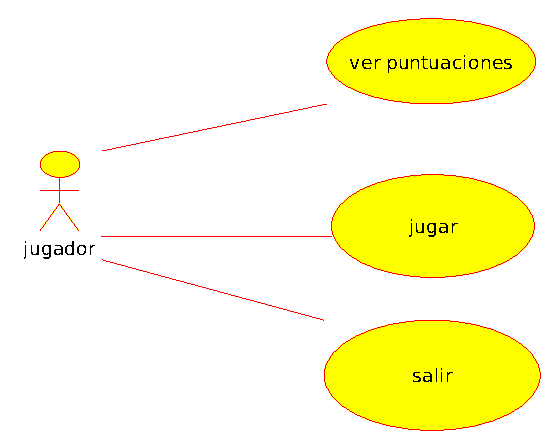
\includegraphics[width = 10 cm]{casos_de_uso_(menu).eps}
\caption{Menú.}
\end{figure}

\begin{figure}[h]
\centering
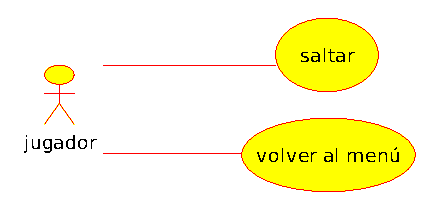
\includegraphics[width = 10 cm]{casos_de_uso_(juego).eps}
\caption{Juego.}
\end{figure}

\clearpage

% -*- coding:utf-8 -*-
\section{Presupuesto}

\begin{itemize}

  \item Costes no recurrentes:

  \begin{itemize}
    \item Registro en Android Market: 18.79 \euro
    \item Equipos portatiles: 4000 \euro (1000 \euro/trabajador, no se incluyen
      para el coste de este proyecto)
    \item Software de desarrollo: 0 \euro (sólo software libre y gratuito)
  \end{itemize}

  \item Costes recurrentes:

  \begin{itemize}

    \item Salario a media jornada: 750 \euro por trabajador/mes

    \begin{itemize}
      \item Sueldo bruto anual: 9000 \euro
      \item Retención IRPF: 0 \euro
      \item Seguridad Social anual: 774.5 \euro
      \item Sueldo Neto anual: 8225.5 \euro
      \item Retención Equivalente: 0 \%
      \item Sueldo neto mensual: 685.46 \euro
      \item Sueldo neto pagas extra: 0 \euro
    \end{itemize}

    \item Proveedor del servicio de internet: 30 \euro por trabajador/mes
    \item Desplazamientos: 40 \euro por trabajador/mes

  \end{itemize}

\end{itemize}

Por tanto, suponiendo un desarrollo a media jornada durante 2 meses, el coste
estimado del proyecto es de {\bf 6578.79 \euro}. Se considera también un fondo
para costes imprevistos de 5000 \euro. Para recuperar la inversión, se
requerirán 7310 descargas a 0.90 \euro.


% \section{Trabajo pendiente.}

% Finalizar el juego añadiendo los elementos que faltan:

% \begin{itemize}
%   \item Menú.
%   \item Cambio del sprite del jugador.
%   \item Si da tiempo, añadir sonido.
% \end{itemize}

% Añadir a este documento los diagramas que faltan.







\section{metodología: PUD + Programación extrema}

-Intro


Resumen de esto ------------------------------
Valores

Los Valores originales de la programación extrema son: simplicidad, comunicación, retroalimentación (feedback) y coraje. Un quinto valor, respeto, fue añadido en la segunda edición de Extreme Programming Explained. Los cinco valores se detallan a continuación:

    Simplicidad:

La simplicidad es la base de la programación extrema. Se simplifica el diseño para agilizar el desarrollo y facilitar el mantenimiento. Un diseño complejo del código junto a sucesivas modificaciones por parte de diferentes desarrolladores hacen que la complejidad aumente exponencialmente. Para mantener la simplicidad es necesaria la refactorización del código, ésta es la manera de mantener el código simple a medida que crece. También se aplica la simplicidad en la documentación, de esta manera el código debe comentarse en su justa medida, intentando eso sí que el código esté autodocumentado. Para ello se deben elegir adecuadamente los nombres de las variables, métodos y clases. Los nombres largos no decrementan la eficiencia del código ni el tiempo de desarrollo gracias a las herramientas de autocompletado y refactorización que existen actualmente. Aplicando la simplicidad junto con la autoría colectiva del código y la programación por parejas se asegura que cuanto más grande se haga el proyecto, todo el equipo conocerá más y mejor el sistema completo.

    Comunicación:

La comunicación se realiza de diferentes formas. Para los programadores el código comunica mejor cuanto más simple sea. Si el código es complejo hay que esforzarse para hacerlo inteligible. El código autodocumentado es más fiable que los comentarios ya que éstos últimos pronto quedan desfasados con el código a medida que es modificado. Debe comentarse sólo aquello que no va a variar, por ejemplo el objetivo de una clase o la funcionalidad de un método. Las pruebas unitarias son otra forma de comunicación ya que describen el diseño de las clases y los métodos al mostrar ejemplos concretos de como utilizar su funcionalidad. Los programadores se comunican constantemente gracias a la programación por parejas. La comunicación con el cliente es fluida ya que el cliente forma parte del equipo de desarrollo. El cliente decide qué características tienen prioridad y siempre debe estar disponible para solucionar dudas.

    Retroalimentación (feedback):

Al estar el cliente integrado en el proyecto, su opinión sobre el estado del proyecto se conoce en tiempo real. Al realizarse ciclos muy cortos tras los cuales se muestran resultados, se minimiza el tener que rehacer partes que no cumplen con los requisitos y ayuda a los programadores a centrarse en lo que es más importante. Considérense los problemas que derivan de tener ciclos muy largos. Meses de trabajo pueden tirarse por la borda debido a cambios en los criterios del cliente o malentendidos por parte del equipo de desarrollo. El código también es una fuente de retroalimentación gracias a las herramientas de desarrollo. Por ejemplo, las pruebas unitarias informan sobre el estado de salud del código. Ejecutar las pruebas unitarias frecuentemente permite descubrir fallos debidos a cambios recientes en el código.

    Coraje o valentía:

Muchas de las prácticas implican valentía. Una de ellas es siempre diseñar y programar para hoy y no para mañana. Esto es un esfuerzo para evitar empantanarse en el diseño y requerir demasiado tiempo y trabajo para implementar todo lo demás del proyecto. La valentía le permite a los desarrolladores que se sientan cómodos con reconstruir su código cuando sea necesario. Esto significa revisar el sistema existente y modificarlo si con ello los cambios futuros se implementaran mas fácilmente. Otro ejemplo de valentía es saber cuando desechar un código: valentía para quitar código fuente obsoleto, sin importar cuanto esfuerzo y tiempo se invirtió en crear ese código. Además, valentía significa persistencia: un programador puede permanecer sin avanzar en un problema complejo por un día entero, y luego lo resolverá rápidamente al día siguiente, sólo si es persistente.

    Respeto:

El respeto se manifiesta de varias formas. Los miembros del equipo se respetan los unos a otros, porque los programadores no pueden realizar cambios que hacen que las pruebas existentes fallen o que demore el trabajo de sus compañeros. Los miembros respetan su trabajo porque siempre están luchando por la alta calidad en el producto y buscando el diseño óptimo o más eficiente para la solución a través de la refactorización del código. Los miembros del equipo respetan el trabajo del resto no haciendo menos a otros, una mejor autoestima en el equipo y elevando el ritmo de producción en el equipo.

----------------------------------------



\subsection{Iteraciones de trabajo}
\textbf{Iteración 0}
16 Febrero Se establece la empresa SHURDROID S.L.
Realizado:
Por hacer: diseño del juego y elección de las herramientas de
desarrollo

\textbf{Iteración 1:}
24 Febrero
Realizado: Terminada la preproducción de juego
Por hacer:
\begin{itemize}
\item Formación de los componentes en Android más AndEngine
\item Primer Game Design Document
\end{itemize}

\textbf{Iteración 2:}
2 Marzo
Realizado: Terminada primera versión de Game Design Document
Por hacer:
\begin{itemize}
\item Pendiente continuar con la formación sobre AndEngine
\item Planificación de siguiente reunión con el supervisor
\end{itemize}

\textbf{Iteración 3:}
8 Marzo
Realizado: Reunión con el supervisor (profesor)
Por hacer:
\begin{itemize}
\item Nueva reunión
\item Tareas del 2 de marzo no terminadas
\end{itemize}

\textbf{Iteración 4:}
18 Marzo
Realizado: ejemplos de práctica
Por hacer: continuar con la formación

\textbf{Iteración 5:}
27 Marzo
Realizado: ejemplos de práctica
Por hacer: continuar con la formación

\textbf{Iteración 6:}
10 Abril
Realizado: ejemplos de práctica
Por hacer: continuar con la formación

\textbf{Iteración 7:}
16 Abril
Realizado: primera versión jugable
Por hacer:
\begin{itemize}
\item Versión alpha para enseñar
\item Siguiente iteración del GDD
\item Reunión con el supervisor
\end{itemize}

\textbf{Iteración 8:}
19 Abril
Realizado:
\begin{itemize}
\item versión alpha
\item siguiente iteración del gdd
\item Reunión con el supervisor
\end{itemize}
Por hacer: Añadir cajas al juego.

\textbf{Iteración 9:}
22 Abril
Realizado:
\begin{itemize}
\item Cajas añadidas.
\item Añadido contador de puntuación.
\end{itemize}
Por hacer: terminar beta del juego

\textbf{Iteración 10:}
29 Abril
Realizado: beta del juego. Se da por concluido el juego a mostrar en
la presentación.
Por hacer: recopilar documentación para la memoria.

\textbf{Iteración 11:}
30 Abril
Realizado: entrega de la memoria.

\subsection{Análisis crítico}
El trabajo entre las iteraciones 0 y 1 se corresponde con la
preproducción del juego. A partir de la iteración 1 comienza el
desarrollo propiamente dicho.

En la siguiente tabla se indica para cada iteración y el porcentaje de trabajo completado
respecto a la previsión de la iteración anterior.



\begin{table}[!ht]
\begin{center}
    \begin{tabular}[!ht]{|c||c|} \hline
      \textbf{Iteración} & \textbf{Porcentaje realizado} \\ \hline
      \textbf{2} & 65 \% \\ \hline
      \textbf{3} & 60 \% \\ \hline
      \textbf{4} & 25 \% \\ \hline
      \textbf{5} & 30 \% \\ \hline
      \textbf{6} & 40 \% \\ \hline
      \textbf{7} & 100 \% \\ \hline
      \textbf{8} & 100 \% \\ \hline
      \textbf{9} & 110 \% \\ \hline
      \textbf{10} & 100 \% \\ \hline
      \textbf{11} & 100 \% \\ \hline
    \end{tabular}
\end{center}
\end{table}


\begin{figure}[h]
\centering
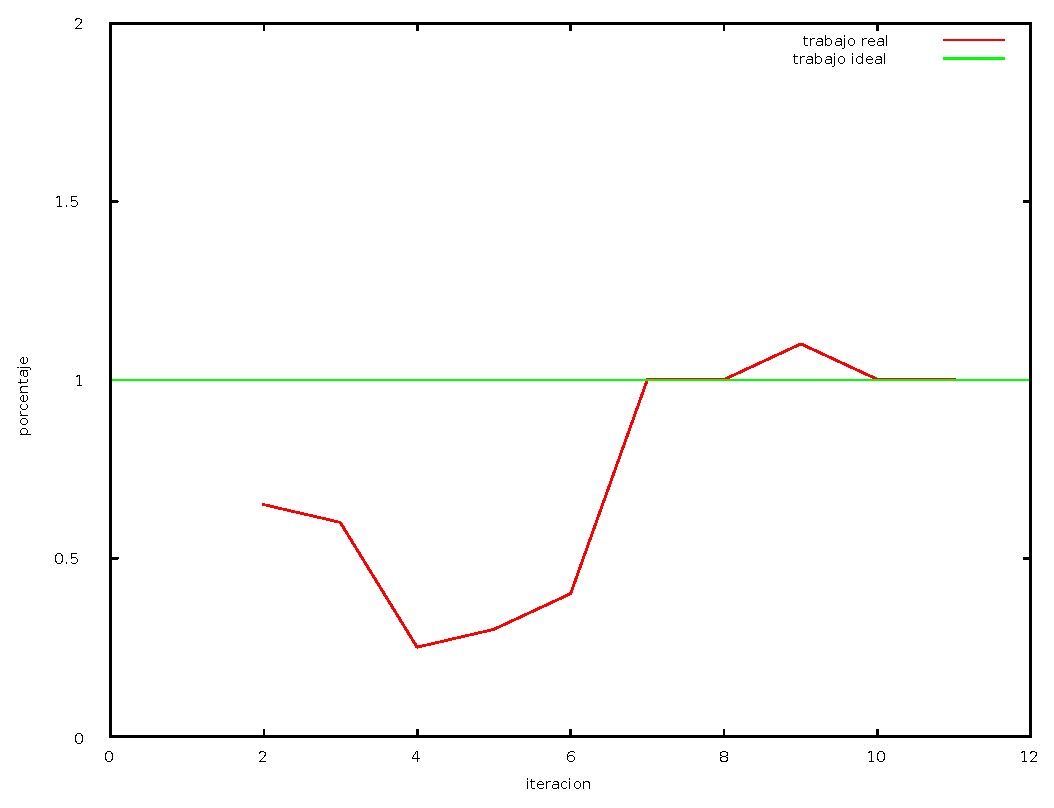
\includegraphics[width = 10 cm]{grafica.eps}
\caption{Gráfica}
\end{figure}


\section{Anexo: estudio de mercado}
Perspectivas

Fácil acceso al mercado, barato el acceso. Android como sistema y
comunidad facilita el desarrollo.

Mucha competencia

Si no estás en el top ten no existes.

Ley de Sturgeon 90\% de todo ES MIERDA

Cierto paralelismo con la época de ora del software español. Con pocos
recursos

Muy premiadas la jugabilidad y la originalidad. Orientado a un mercado
de jugadores casuales, con una interfaz fácil y que pueda jugarse
pocos minutos.

Se puede enfocar como un primer escalón en consolidad tu empresa como
desarrolladora de juegos de otros tipos, como X-Box live, Steam o ser
contratado por empresas mayores del mercado.

Es decir, algo como un estudio de mercado viendo:
qué competencia hay,
 qué probabilidad se estima de que la empresa sobreviva,
qué probabilidad hay de tener un gran éxito o si es más probable ir sobreviviendo entre la competencia, etc.


\section{Fuentes}
\href{http://www.android.com}{Android}

\href{http://developer.android.com/index.html}{Android Developer}

\href{http://www.andengine.org/}{AndEngine}

\href{https://github.com/nicolasgramlich/AndEngine}{AndEngine github repository}

\href{http://droideando.blogspot.com.es}{Droideando blogspot}

\end{document}
